
\chapter{Introduction/A First Level Heading}
\section{A Second-Level Heading}

\lipsum[35]\\ 

\lipsum[26]


\section{Another Second Level Heading, But This One Is So Long That It Needs to Take Up Multiple Lines}
\lipsum[45]

\vspace{2\baselineskip}
\begin{figure}[htb!]
    \caption{Word Cloud of Lorem Ipsum Paragraph.}
    
    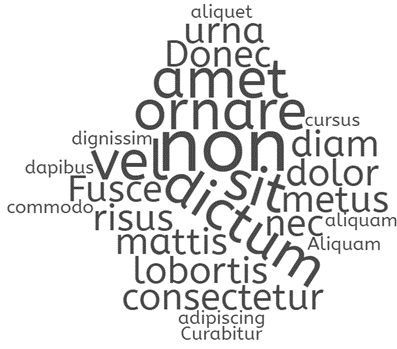
\includegraphics[width = 4in]{Figures/word_cloud.png}
    \label{fig: word cloud}
\end{figure}
\FloatBarrier
\vspace{\baselineskip}

\lipsum[78]

\subsection{A Third Level Heading}

\lipsum[2]

\subsubsection{A Fourth Level Heading.}\lipsum[9]

\paragraph{A Fifth Level Heading. } \lipsum[11]

\vspace{2\baselineskip}
\begin{table}[hp!]
\caption{A Table That Breaks Over Two Pages}
\begin{tabular}{l|l|l|l|}
\cline{2-4}
                                              & \textbf{Column Heading 1} & \textbf{Column Heading 2} & \textbf{Column Heading 3} \\ \hline
\multicolumn{1}{|l|}{\textbf{Row Heading 1}}  &                           &                           &                           \\ \hline
\multicolumn{1}{|l|}{\textbf{Row Heading 2}}  &                           &                           &                           \\ \hline
\multicolumn{1}{|l|}{\textbf{Row Heading 3}}  &                           &                           &                           \\ \hline
\multicolumn{1}{|l|}{\textbf{Row Heading 4}}  &                           &                           &                           \\ \hline
\multicolumn{1}{|l|}{\textbf{Row Heading 5}}  &                           &                           &                           \\ \hline
\multicolumn{1}{|l|}{\textbf{Row Heading 6}}  &                           &                           &                           \\ \hline
\multicolumn{1}{|l|}{\textbf{Row Heading 7}}  &                           &                           &                           \\ \hline
\multicolumn{1}{|l|}{\textbf{Row Heading 8}}  &                           &                           &                           \\ \hline
\multicolumn{1}{|l|}{\textbf{Row Heading 9}}  &                           &                           &                           \\ \hline
\multicolumn{1}{|l|}{\textbf{Row Heading 10}} &                           &                           &                           \\ \hline
\multicolumn{1}{|l|}{\textbf{Row Heading 11}} &                           &                           &                           \\ \hline
\end{tabular}
\end{table}
\FloatBarrier


\newpage
\begin{table}[htpb]
\begin{tabular}{l|l|l|l|}
\cline{2-4}
                                              & \textbf{Column Heading 1} & \textbf{Column Heading 2} & \textbf{Column Heading 3} \\ \hline
\multicolumn{1}{|l|}{\textbf{Row Heading 12}}  &                           &                           &                           \\ \hline
\multicolumn{1}{|l|}{\textbf{Row Heading 13}}  &                           &                           &                           \\ \hline
\multicolumn{1}{|l|}{\textbf{Row Heading 14}}  &                           &                           &                           \\ \hline

\end{tabular}
\end{table}
\FloatBarrier
\vspace{\baselineskip}

\lipsum[55] \\

\lipsum[42] This is an example of what a block quote will look like:

\begin{adjustwidth}{2.5em}{0pt}
This is a block quote. It is indented once, using the Increase Indent button, and it is always double spaced. \lipsum[1]
\end{adjustwidth}

\lipsum[21]\\
 
\lipsum[12]

\section{How Equations Should Look in Your Document}
\lipsum[1]

\begin{equation}\label{eq: nchoosek}
    (x+a)^n = \sum_{k = 0}^n \binom{n}{k} x^k a^{n-k}  
\end{equation}

\vspace{12pt}

Reference equation \ref{eq: nchoosek}. \lipsum[63]\\

\lipsum[62]

\vspace{2\baselineskip}
\begin{table}[ht!]
\caption{Most Tables Have Short, Capitalized Titles}

\begin{tabular}{|L{0.4\textwidth}|L{0.4\textwidth}|}
\hline
Data         & \textbf{More Data} \\ \hline
\textbf{Yes} & 70\%               \\ \hline
\textbf{No}  & 30\%               \\ \hline
\end{tabular}


\medskip
\small\textit{Note}. 
\begin{doublespace}
If there is more information that needs to be provided for context or to explain the data, then it should be included either in the paragraph that refers to the table or, if it doesn’t fit there, in a note below the table, formatted just like this one, with the word “Note” italicized and followed by a period, and the note itself double-spaced.
\end{doublespace}
\end{table}
\FloatBarrier
\vspace{\baselineskip}

\lipsum[2]

